\documentclass[a4paper,10pt]{scrreprt}
\usepackage[top=2cm,bottom=4cm]{geometry}
\usepackage[english]{babel}
\usepackage[T1]{fontenc}  			% make sure to install cm-super package for improved PDF quality
\usepackage[utf8]{inputenc}
\usepackage{lmodern}
%\usepackage[cm]{fullpage}			% Fullpage for now
\usepackage{graphicx}
\usepackage[dvipsnames]{xcolor}
\usepackage[font=small]{caption}
\usepackage{subcaption}
\usepackage{microtype}			 	% microtypographical fine-tunning
\usepackage{setspace} 				% Provides support for setting the spacing between lines in a document.
%\usepackage{tocbibind}				% Add bibliography/index/contents to Table of Contents.
\usepackage{mathtools}				% enhances amsmath (no need to load amsmath)
\usepackage{amssymb}
\usepackage{amsfonts}
\usepackage{amsthm}
\usepackage{bm} 					% bold math symbols including greek letters
\usepackage{booktabs}				% professional tables (w/o vertical bars)
\usepackage{array}					% 
\usepackage{dcolumn} 				% align to decimal point in tables
\usepackage[shortcuts]{extdash} 	% hyphenation of dashed words
%\usepackage[algoruled]{algorithm2e}
%\newcommand\mycommfont[1]{\small\ttfamily #1}
%\SetCommentSty{mycommfont}
\usepackage{cleveref}				% clever environment referencing
\crefname{figure}{Fig.}{Figs.}
\crefname{algorithm}{Alg.}{Algs.}
\usepackage{siunitx}				% typesetting of SI units
%\usepackage{paralist}		     	% compact lists with more options
%\usepackage[]{todonotes}			% TODO notes
%\presetkeys{todonotes}{backgroundcolor=orange!50}{}
% Not sure which to use for bibliography
%\usepackage{cite}
%\usepackage{citesort}
\usepackage[square, sort, numbers, authoryear]{natbib}
\usepackage{physics}

% ======================== MACROS ==========================
% TODO and other notes
\DeclareDocumentCommand \note 		{ m }{ \textcolor{OrangeRed}{\ \\ \emph{\textbf{(NOTE)}} #1}\ \\ }

% MATH OPERATORS ===============================================================
\DeclareMathOperator*{\argmin}{ \arg\min }
\DeclareMathOperator{\atantwo}{\mathrm{atan2}}
\DeclareMathOperator{\sign}{\mathrm{sign}}
\DeclareMathOperator{\vect}{vec}
\DeclareMathOperator{\pdeg}{pdeg}

% BASIC MACROS =================================================================
% Bold vector and matrix
\DeclareDocumentCommand \vb{ s m } {
	\IfBooleanTF #1 {
		\bm{\lowercase{#2}}
	}{
		\bm{\mathbf{\lowercase{#2}}}
	}
}
\DeclareDocumentCommand \mb { s m } {
	\IfBooleanTF #1 {
		\bm{\uppercase{#2}}
	}{
		\bm{\mathbf{\uppercase{#2}}}
	}
}
% Matrix inverse and transpose
\DeclareDocumentCommand \I		{}{ ^{-1} }
\DeclareDocumentCommand \T		{}{ ^{\top} }
% Diagonal matrix
\DeclareDocumentCommand \diag 	{ l m }{ \mathrm{diag}\pqty#1{\, #2 \,} }
% Unit matrix
\DeclareDocumentCommand \eye 	{ }{ \mb{I} }
% zero vector
\DeclareDocumentCommand \vzero  { }{ \vb{0} }
% elementary vector
\DeclareDocumentCommand \eVec  	{ }{ \vb{e} }
% unit vector
\DeclareDocumentCommand \uVec  	{ }{ \vb{1} }
% column operator
\DeclareDocumentCommand \col  	{ m m }{ \bqty{#1}_{*#2} }
% Integral sign and differential
\DeclareDocumentCommand \integ 	{ O{} O{} }{ \int\limits_{#1}^{#2}\! }
\DeclareDocumentCommand \iinteg { O{} O{} }{ \iint\limits_{#1}^{#2}\! }
\DeclareDocumentCommand \iiinteg{ O{} O{} }{ \iiint\limits_{#1}^{#2}\! }
\DeclareDocumentCommand \dx 	{ O{x} }{ \,\mathrm{d}#1 }
% Expectation, variance and covariance
\DeclareDocumentCommand \E 		{ O{} l m }{ \mathbb{E}_{#1}\bqty#2{ #3 } }
\DeclareDocumentCommand \V 		{ O{} l m }{ \mathbb{V}_{#1}\bqty#2{ #3 } }
\DeclareDocumentCommand \Cov 	{ O{} l m }{ \mathbb{C}_{#1}\bqty#2{ #3 } }
% Kullback-Leibler divergence
\DeclareDocumentCommand \KL 	{ m m }{ \mathbb{KL} \bqty{\left. #1 \,\middle\|\, #2 \right.} }
% Density of Gaussian, Student's t, Gamma and Inverse Gamma variable
\DeclareDocumentCommand \N 		{ s O{\vb{x}} O{\vb{0}} O{\eye} }
{
	\IfBooleanTF{#1}{
		#2\sim\mathrm{N}\pqty{ #3,\, #4 }
	}{
		\mathrm{N}\pqty{\left. #2 \,\middle\vert\, #3,\, #4 \right.}
	}
}
\DeclareDocumentCommand \pdfc	{ O{p} m m }
{
	#1\pqty{\left. #2 \,\middle\vert\, #3 \right.} 
}

% STATE ESTIMATION =============================================================
% time index and final time index
\DeclareDocumentCommand	\tind		{ }{ k }
\DeclareDocumentCommand	\Tind		{ }{ K }
% general nonlinear fcn, system dynamics and measurement fcn
\DeclareDocumentCommand \nlFcn 		{ s }{ \IfBooleanTF{#1}{g}{\vb{g}} }
\DeclareDocumentCommand \stFcn		{  }{ \vb{f} }
\DeclareDocumentCommand \msFcn		{  }{ \vb{h} }
% Jacobian
\DeclareDocumentCommand \jacb 		{ m }{ \mb{g}\pqty{#1} }
% state and measurement variables
\DeclareDocumentCommand \stVar 		{ s }{ \IfBooleanTF{#1}{x}{\vb{x}} }
\DeclareDocumentCommand \msVar		{ s }{ \IfBooleanTF{#1}{z}{\vb{z}} }
% state and measurement noise
\DeclareDocumentCommand \stnVar		{ s }{ \IfBooleanTF{#1}{q}{\vb{q}} }  % TODO rename to \snVar, \stnVar
\DeclareDocumentCommand \msnVar		{ s }{ \IfBooleanTF{#1}{r}{\vb{r}} }
% state and measurement noise covariances
\DeclareDocumentCommand \stnCov		{ s }{ \IfBooleanTF{#1}{\sigma^2_q}{\mb{Q}} }
\DeclareDocumentCommand \msnCov		{ s }{ \IfBooleanTF{#1}{\sigma^2_r}{\mb{R}} }
% state and measurement mean, covariance and cross-covariance
\DeclareDocumentCommand \stMean		{   }{ \vb{m}^x }
\DeclareDocumentCommand \msMean		{   }{ \vb{m}^z }
\DeclareDocumentCommand \stCov		{   }{ \mb{P}^x }
\DeclareDocumentCommand \stMsCov	{   }{ \mb{P}^{xz} }
\DeclareDocumentCommand \msStCov	{   }{ \mb{P}^{zx} }
\DeclareDocumentCommand \msCov		{   }{ \mb{P}^z }
% multi-state, multi-measurement
\DeclareDocumentCommand \mstVar 	{   }{X}
\DeclareDocumentCommand \mmsVar 	{   }{Z}
% filtered state mean and covariance
\DeclareDocumentCommand \filtMean 	{ O{\tind} }{ \stMean_{#1|#1} }
\DeclareDocumentCommand \filtCov 	{ O{\tind} }{ \stCov_{#1|#1} }
% Kalman gain
\DeclareDocumentCommand \kGain		{  }{ \mb{K} }
% input and output dimension
\DeclareDocumentCommand \inDim 		{  }{ D }
\DeclareDocumentCommand \outDim 	{  }{ E }
% state and measurement dimension
\DeclareDocumentCommand \stDim 		{  }{ {d_x} }
\DeclareDocumentCommand \msDim 		{  }{ {d_z} }
\DeclareDocumentCommand \stnDim 	{  }{ {d_q} }
\DeclareDocumentCommand \msnDim		{  }{ {d_r} }
% general decoupled input variable, input variable, output variable
\DeclareDocumentCommand \inVar 		{ s }{ \IfBooleanTF{#1}{{x}}{{\vb{x}}} }
\DeclareDocumentCommand \inVarU		{ s }{ \IfBooleanTF{#1}{{\xi}}{{\vb{\xi}}} }
\DeclareDocumentCommand \inVarC		{ s }{ \IfBooleanTF{#1}{{\eta}}{{\vb{\eta}}} }
\DeclareDocumentCommand \outVar 	{ s }{ \IfBooleanTF{#1}{y}{\vb{y}} }
% input mean, covariance, cov. square-root
\DeclareDocumentCommand \inMean 	{  }{ \vb{m} }
\DeclareDocumentCommand \inCov 		{  }{ \mb{P} }
\DeclareDocumentCommand \inCovFct	{  }{ \mb{L} }
% output mean, covariance and cross-covariance
\DeclareDocumentCommand \outMean 	{  }{ \vb{\mu} }
\DeclareDocumentCommand \outCov 	{  }{ \mb{\Pi} }
\DeclareDocumentCommand \inoutCov 	{  }{ \mb{C} }
% approximate output mean, covariance and cross-covariance
\DeclareDocumentCommand \outMeanApp	{  }{ \vb{\mu}_{\mathrm{A}} }
\DeclareDocumentCommand \outCovApp 	{  }{ \mb{\Pi}_{\mathrm{A}} }
\DeclareDocumentCommand \inoutCovApp{  }{ \mb{C}_{\mathrm{A}} }
% set of reals, naturals, dataset, state space, measurement space
\DeclareDocumentCommand \R 			{  }{ \mathbb{R} }
\DeclareDocumentCommand \Nat		{  }{ \mathbb{N} }
\DeclareDocumentCommand \D 			{  }{ \mathcal{D} }
\DeclareDocumentCommand \Cinf		{  }{ \mathcal{C}^{\infty} }
\DeclareDocumentCommand \stSp		{  }{ \mathcal{X} }
\DeclareDocumentCommand \msSp		{  }{ \mathcal{Z} }
% degrees of freedom parameter: arbitrary, TPQ related and a Student update related
\DeclareDocumentCommand \inDof 		{  }{ \nu }
\DeclareDocumentCommand \nlfDof 	{  }{ \nu_{\nlFcn*} }
\DeclareDocumentCommand \stDof 		{  }{ \nu^x }
\DeclareDocumentCommand \msNoiseDof	{  }{ \nu^r }
\DeclareDocumentCommand \stNoiseDof	{  }{ \nu^q }
\DeclareDocumentCommand \filtDof 	{ O{\tind} }{ \stDof_{#1|#1} }
\DeclareDocumentCommand \fixDof 	{ O{\tind} }{ \nu^* }

% RANDOM FINITE SET FILTERING ===================================
% set differential
\DeclareDocumentCommand \dsx	{ O{X} }{ \mathrm{\delta}#1 }
% multi-targte state related quantities
\DeclareDocumentCommand \stSet	{ }{ X }
\DeclareDocumentCommand \stRFS	{ }{ X }
% set of measurements
\DeclareDocumentCommand \msSet	{ }{ Z }
\DeclareDocumentCommand \msRFS	{ }{ Z }



% ======================== THEOREMS ========================
\theoremstyle{theorem}
\newtheorem{thm}{Theorem}
\newtheorem{lem}{Lemma}
\newtheorem{cor}{Corollary}
\theoremstyle{definition}
\newtheorem{defn}{Definition}
\newtheorem{alg}{Algorithm}
% ========================================================


% Title Page
\title{Notes on Multi-target Tracking}
\author{Jakub Prüher}


\begin{document}
%\maketitle

%\begin{abstract}
%	This report summarizes my understanding of the multi-target tracking (MTT) problems and the most representative algorithms. 
%	First, I cover prerequisites necessary for understanding multi-target tracking such as basics of single-target tracking (Bayesian filtering), measurement formation and data association.
%	The aim is to describe the most representative MTTs, such as joint probabilistic data association filter (JPDAF), multiple hypothesis tracking (MHT) and finally, my favourite, random finite set (RFS) approaches.
%\end{abstract}


%\chapter{Prerequisites}\label{ch:prerequisites}
%\section{Single-Target Tracking}\label{sec:single-target_tracking}
%\section{Single-Target Tracking in Clutter}\label{sec:single-target_tracking_in_clutter}
%\section{Data Association}\label{sec:data_association}
%Global nearest neighbor (GNN)\\
%All-neighbors data association - broader concept, PDA is a special case\\
%Gating - 
%\subsection{Probabilistic Data Association}
%\chapter{Joint Probabilistic Data Association Filter}\label{ch:jpda_filter}
%\chapter{Multiple Hypothesis Tracking}\label{ch:multiple_hypothesis_tracking}


\chapter{Random Finite Sets}\label{ch:random_finite_sets}
% NOTE: the convention that upper-case letters denote number of elements and lower-case counterpart indexes the elements needs to be abandoned, because upper-case is now reserved for RVs and lower-case for RV realizations.
% Thus, N = discrete random variable, n = realization of N (= number of elements in RFS X)

\begin{defn}[\emph{Set Integral}]
	 of a set function \( \pi \) is defined as
	\begin{equation}\label{eq:set_integral}
		\int_S \pi(X) \dsx[X] \triangleq \sum_{k=0}^{\infty}\frac{1}{k!}\int_{S^k} \pi(\Bqty{\inVar_1, \inVar_2, \ldots, \inVar_k}) \dx[(\inVar_1, \inVar_2, \ldots, \inVar_k)]
	\end{equation}
	with the convention \( \int_{S^0} \pi(\emptyset) \dsx[\emptyset] = \pi(\emptyset) \).
\end{defn}

\begin{defn}[\emph{FISST Density}]
	 is a set function \( \pi(X) \) such that 
	\begin{equation}\label{eq:fiist_density}
		\Pr(S \subseteq \mathcal{X}) = \int_S \pi(X) \dsx[X]
	\end{equation}
\end{defn}
FISST density \emph{is not} a probability density.

\begin{defn}[\emph{Cardinality Distribution}]
	Cardinality distribution of a RFS \( X \) is given by
	\begin{equation}\label{key}
		\rho(n) = \Pr(|X|=n) = \frac{1}{n!}\int \pi(\Bqty{\stVar_1,\, \ldots,\, \stVar_n}) \dx[\stVar_1]\cdot\ldots\cdot\dx[\stVar_n]
	\end{equation}
	It's nothing but a probability mass function (PMF) of a discrete random variable \( N \sim \rho(n) \).
\end{defn}

\begin{defn}[\emph{I.I.D. Cluster RFS}]
	RFS \( X \) of cardinality \( n \) with FISST density
	\begin{equation}\label{key}
		\pi(X) = n! \rho(n) \prod_{i=1}^{n} p(\stVar_i).
	\end{equation}
	The RFS contains elements \( \stVar_1, \ldots, \stVar_n \) that are i.i.d. according to a probability density \( p(\stVar): \stSp\to\R \).
\end{defn}

\begin{defn}[\emph{Poisson RFS}]
	I.I.D cluster with Poisson cardinality density, that is
	\begin{equation}\label{key}
		\rho(n \mid \lambda) = e^{-\lambda} \frac{\lambda^n}{n!}
	\end{equation}
	where \( \lambda \) is the expected number of objects.
	Poisson RFS is completely describes by its intensity function.
\end{defn}

\begin{defn}[\emph{Bernoulli RFS}]
\begin{equation}\label{eq:bernoulli_rfs}
	\pi(X) = 
	\begin{cases}
	1 - r, 			& X = \emptyset \\
	r p(\stVar), 	& X = \Bqty{\stVar}
	\end{cases}
\end{equation}
\end{defn}

\begin{defn}[\emph{Multi-Bernoulli RFS}]
	Union of independent Bernoulli RFSs.
\end{defn}

\begin{defn}[\emph{Probability Hypothesis Density}]
	For a RFS \( X \) and , the intensity function is defined as
	\begin{equation}\label{key}
		v(\stVar) = \int \pi(\Bqty{\stVar} \cup X) \dsx[X]
	\end{equation}
	Integrating intensity over a (deterministic) subset of state space \( S \subseteq \mathcal{X} \) yields the expected number of elements (expected cardinality) in \( S \)
	\begin{equation}\label{key}
		\E{|X \cap S|} = \int_S v(\stVar) \dx[\stVar]
	\end{equation}
\end{defn}
Probability hypothesis density (PHD) is also known as intensity function.

\begin{figure}[h]
	\centering
	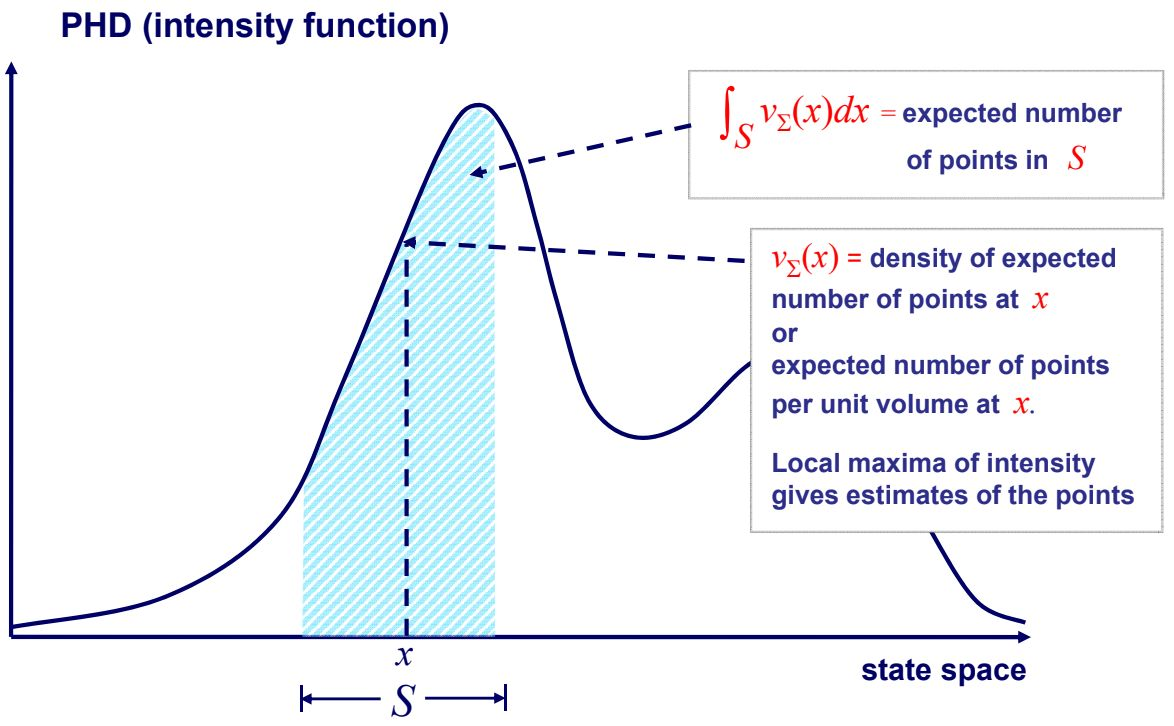
\includegraphics[scale=0.22]{./img/intensity_function}
	\caption{Intensity function, a.k.a. probability hypothesis density (PHD).}
\end{figure}




\section{Multi-target State-Space Models}

Let $ \pi(\cdot \mid \msSet_{1:\tind}) $ denote the multi-target posterior density.
Then, the optimal multi-target Bayes filter propagates the multi-target posterior in time via the recursion

\begin{align}
	\pi(\stSet_\tind \mid \msSet_{1:\tind-1}) 
	&= \integ \stFcn(\stSet_\tind \mid \stSet_{\tind-1}) \pi(\stSet_{\tind-1} \mid \msSet_{1:\tind-1}) \mu(\dx[\stSet_{\tind-1}]) \\
	\pi(\stSet_\tind \mid \msSet_{1:\tind}) 
	&= \frac{\msFcn(\msSet_\tind \mid \stSet_\tind) \pi(\stSet_\tind \mid \msSet_{1:\tind-1})}{\integ \msFcn(\msSet_\tind \mid \stSet_\tind) \pi(\stSet_\tind \mid \msSet_{1:\tind-1}) \mu(\dx[\stSet_\tind])}
\end{align}


\begin{figure}[h]
	\centering
	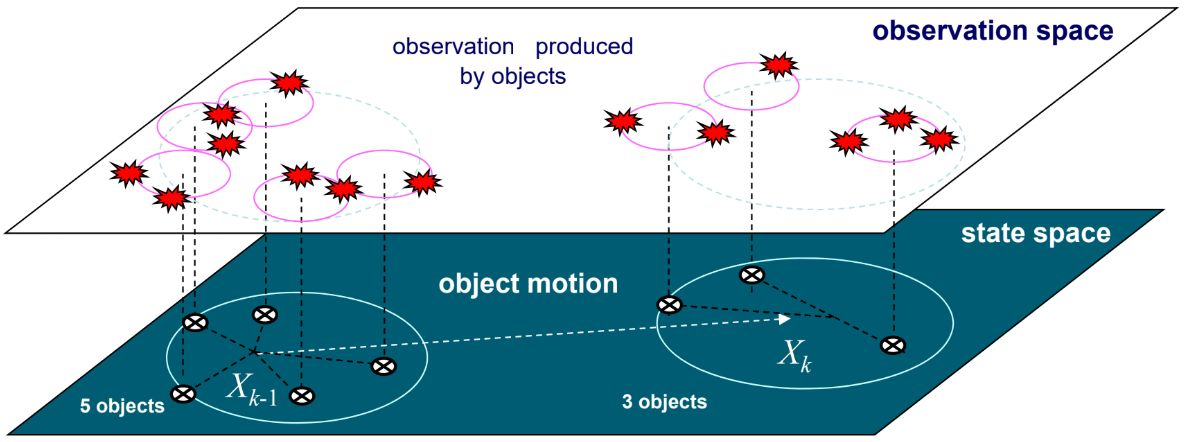
\includegraphics[scale=0.25]{./img/multi-target_state_space_model}
	\caption{Multi-target state space model.}
\end{figure}

\subsection{Motion model}
Given a multi-target state \( \stRFS_{\tind-1} \) at time \( \tind-1 \), the multi-target state \( \stRFS_\tind \) at time \( \tind \) is given by the union of the surviving targets, the spawned targets and the spontaneous births
\begin{equation}\label{eq:multitarget_dynamics}
	\stRFS_\tind = \bqty{ \bigcup_{\vb{\zeta} \in \stRFS_{\tind-1}} S_{\tind|\tind-1}(\vb{\zeta}) } \cup \bqty{ \bigcup_{\vb{\zeta} \in \stRFS_{\tind-1}} B_{\tind|\tind-1}(\vb{\zeta}) } \cup \Gamma_\tind
\end{equation}
where
\begin{table}[h]
\centering
\begin{tabular}{@{} l l @{}}
	\toprule
	\( S_{\tind|\tind-1}(\vb{\zeta}) \)		& RFS modeling the behaviour of a target at time step \( \tind \) given a state at time \( \tind-1 \); \\
											& takes on the value \( \Bqty{\inVar_\tind} \) when target survives, or \( \emptyset \) when the target dies. \\
	\( B_{\tind|\tind-1}(\vb{\zeta}) \)		& RFS of targets spawned at time \( \tind \) from a target with previous state \( \vb{\zeta} \) \\
	\( \Gamma_\tind \)						& RFS of spontaneous birth at time \( \tind \) \\
	\bottomrule
\end{tabular}
\end{table}
The actual forms of \( B_{\tind|\tind-1}(\cdot) \) and \( \Gamma_\tind \) are problem dependent.
\begin{figure}[h]
	\centering
	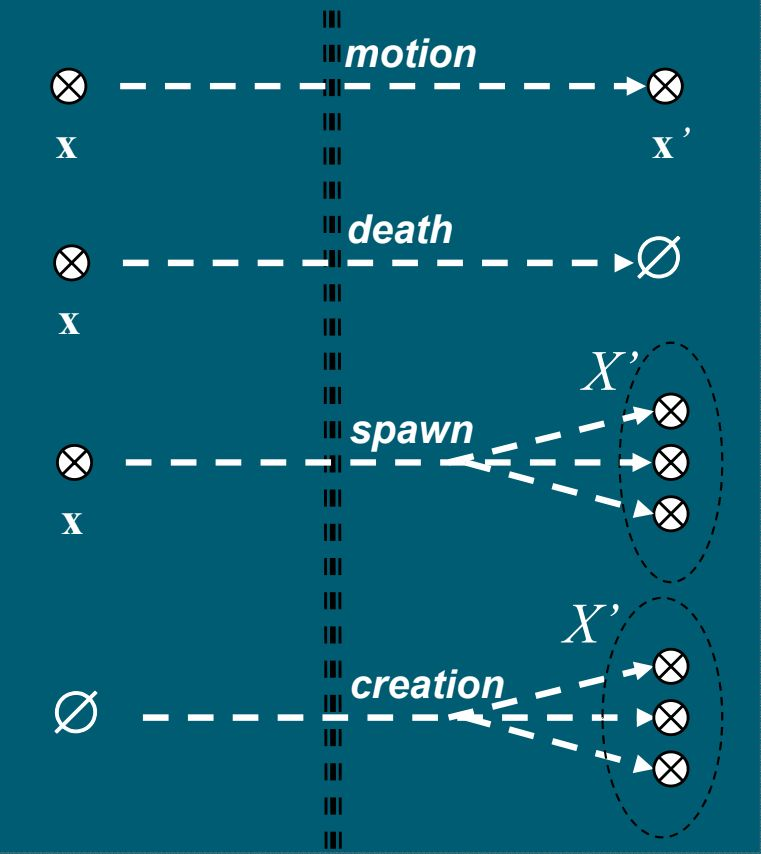
\includegraphics[scale=0.2]{./img/multi-target_motion_model}
	\caption{Multi-target motion model.}
\end{figure}

\subsection{Observation model}
\begin{equation}\label{eq:multitarget_observation}
	\msRFS_\tind = \bqty{ \bigcup_{\vb{\zeta} \in \stRFS_{\tind-1}} \Theta_{\tind}(\inVar) } \cup K_\tind
\end{equation}
where
\begin{table}[h]
	\centering
	\begin{tabular}{@{} l l @{}}
		\toprule
		\( \Theta_{\tind}(\inVar) \)	& RFS generated by the state at time $ \tind $; takes on \( \Bqty{\msVar_\tind} \) when \\ 
										& the target is detected, or \( \emptyset \) when the target is not detected, \\
		\( K_\tind \)					& clutter (false measurements/alarms) \\
		\bottomrule
	\end{tabular}
\end{table}
The actual form of \( K_\tind \) is problem dependent.
\begin{figure}[h]
	\centering
	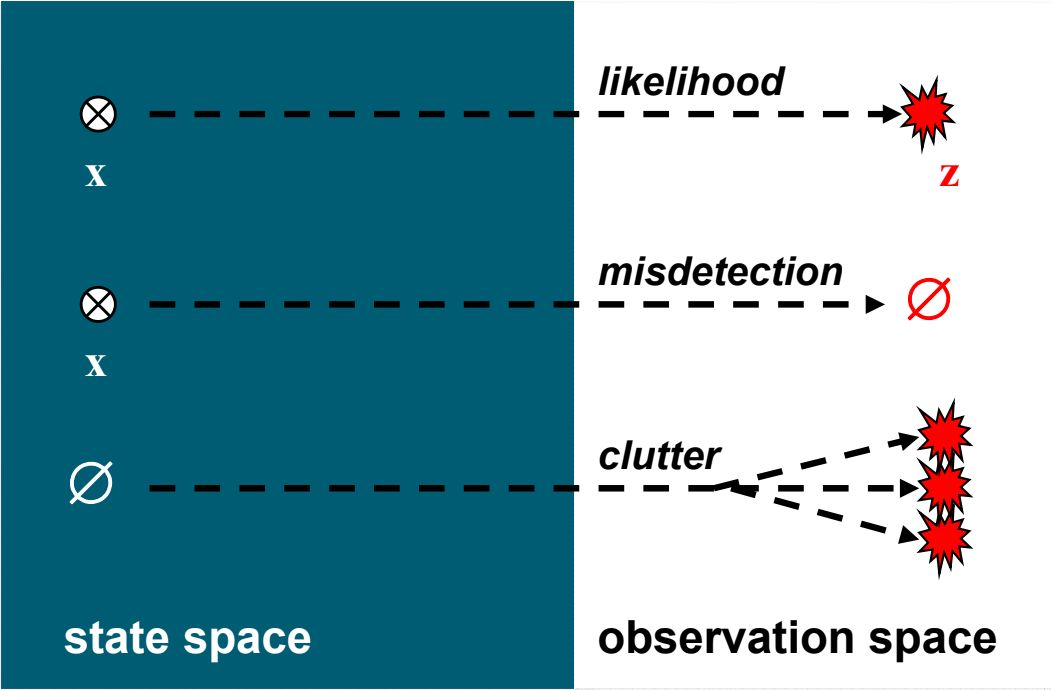
\includegraphics[scale=0.22]{./img/multi-target_observation_model}
	\caption{Multi-target observation model.}
\end{figure}




\section{Probability Hypothesis Density Filter}
Propagates only the first moment of the RFS.

\begin{table}[h]
\centering
\begin{tabular}{@{} l l @{}}
	\toprule
	\( \gamma_\tind(\cdot) \)								& intensity of the birth RFS \( \Gamma_\tind \) at time \( \tind \) \\
	\( \beta_{\tind|\tind-1}(\cdot \mid \vb{\zeta}) \) 		& intensity of the RFS \( B_{\tind|\tind-1}(\vb{\zeta}) \) spawned at time \( \tind \) by a target with previous state \( \vb{\zeta} \) \\
	\( \kappa_\tind(\cdot) \)								& intensity of the clutter RFS \( K_\tind \) at time \( \tind \) \\
	\( p_{S,k}(\vb{\zeta}) \)								& probability of target survival at time \( \tind \) given that its previous state is \( \vb{\zeta} \) \\
	\( p_{D,k}(\inVar) \)									& probability of target detection at time \( \tind \) given a state \( \inVar \) \\
	\bottomrule
\end{tabular}
\end{table}

\ \\
\textbf{Assumptions}\\
\begin{description}
	\item[A1] Each target evolves and generates observations independently of one another,
	\item[A2] Clutter is Poisson and independent of target-originated measurements,
	\item[A3] The predicted multi-target RFS governed by \( p_{\tind|\tind-1} \) is Poisson.
\end{description}


Prediction
\begin{equation}\label{eq:phd_filter_prediction}
	v_{\tind|\tind-1}(\inVar) 
	= \integ p_{S,\tind}(\vb{\zeta}) \stFcn_{\tind|\tind-1}(\inVar \mid \vb{\zeta}) v_{\tind-1}(\vb{\zeta}) \dx[\vb{\zeta}]
	+ \integ \beta_{\tind|\tind-1}(\inVar \mid \vb{\zeta}) v_{\tind-1}(\vb{\zeta}) \dx[\vb{\zeta}] + \gamma_\tind(\inVar)
\end{equation}

measurement update
\begin{equation}\label{eq:phd_filter_update}
	v_\tind(\inVar) = (1 - p_{D,\tind}(\inVar))v_{\tind|\tind-1}(\inVar) + \sum\limits_{\msVar \in \msSet_\tind} \frac{p_{D,\tind}(\inVar)\msFcn_\tind(\msVar \mid \inVar) v_{\tind|\tind-1}(\inVar)}{\kappa_\tind(\msVar) + \integ p_{D,\tind}(\inVarU) \msFcn_\tind(\msVar\mid\inVarU) v_{\tind|\tind-1}(\inVarU) \dx[\inVarU]} 
\end{equation}



\subsection{Gaussian Mixture Probability Hypothesis Density Filter (GM-PHD)}\label{ssec:gaussian_mixture_phd_filter}
Assumes the intensity function has the form of Gaussian mixture.
Merging and pruning required to curb the exponential explosion of mixture components.

\section{Cardinalized Probability Hypothesis Density Filter}\label{sec:cardinalized_phd_filter}
In addition to propagating the intensity function, CPHD also propagates the cardinality distribution of the RFS.

\section{Multi-Bernoulli Filter}
Precursor to LMB filter, which I wanna learn to get to the LMB SLAM.
State RFSs are multi-Bernoulli. 
I don't know what that means practically.




\chapter{Labeled Random Finite Sets}\label{ch:labeled_random_finite_sets}
PHD, CPHD filters do not tell you the track identity and thus tracks can't be told apart. 
So for example, if there are two tracks that cross each other and third one gets born right at their intersection a potential confusion might arise as to continuity of each track.
Useful for designing multi-target filters that produce labeled trajectories, which is ultimately what we really want.

\section{Labeled Multi-Bernoulli Filter}\label{sec:labeled_multi-bernoulli_filter}
LMB filter



\bibliographystyle{plainnat}
\bibliography{refdb}
\end{document}          
